
%(BEGIN_QUESTION)
% Copyright 2014, Tony R. Kuphaldt, released under the Creative Commons Attribution License (v 1.0)
% This means you may do almost anything with this work of mine, so long as you give me proper credit

Calculate the primary winding current (magnitude and phase angle) for this resistively loaded isolation transformer, with primary and secondary inductances of 18 Henrys each:

$$\includegraphics[width=15.5cm]{i01252x01.eps}$$

Also, draw an equivalent schematic diagram (with no transformer in it) illustrating the impedance ``seen'' by the AC power source.  Assume no winding resistance in either transformer winding, and a magnetic coupling coefficient between the two windings of exactly 1.

\underbar{file i01252}
%(END_QUESTION)





%(BEGIN_ANSWER)

$I_{primary} = 1.2001 \hbox{ A} \> \angle -0.84^o$

$$\includegraphics[width=15.5cm]{i01252x02.eps}$$

%(END_ANSWER)





%(BEGIN_NOTES)

This question illustrates how reflected load impedance is ``seen'' by the source, and how it interacts with the transformer's intrinsic winding impedance.

%INDEX% Electronics review: transformer ratios

%(END_NOTES)


